\section{Auswertung}
\label{sec:Auswertung}
\subsection{Mathematische Methoden}
In der folgenden Auswertung wurden die arithmetischen Mittel mit der
Gleichung
\begin{equation}
  \bar{x} \coloneq \frac{1}{n} \sum_{i=1}^n x_i
  \label{eqn:aM}
\end{equation}
brechnet, dabei bezeichnet $\bar{x}$ das arithmetische Mittel, $n$ die Anzahl
der Messwerte und $x_i$ die einzelnen Messwerte. \\
Die Ausgleichsrechnungen, auch Fits genannt, wurden im folgenden mit der
Formel
\begin{equation}
  \increment \nu \stackrel{!}{=} f(x) = a\cdot v
  \label{eqn:fit}
\end{equation}
getätigt. Dabei bezeichnet $\increment \nu$ die Frequenzänderung, $v$ die
Geschwindigkeit und $a$ ist der zu berechnende Proportionalitätsfaktor zwischen
$ \increment \nu $ und $v$ . Laut Versuchsanleitung \cite{Anleitung} gilt für den
Proportionalitätsfaktor $a$ der Zusammenhang
\begin{equation}
  \increment \nu = a\cdot v = v\cdot\frac{\nu_0}{c} \quad \text{daraus folgt} \quad
  a = \frac{\nu_0}{c}
  \label{eqn:a}
\end{equation}
\\
Relative Fehler werden im folgenden mit der Formel
\begin{equation*}
  \increment x = \frac{\lvert x_e - x_m \rvert}{\lvert x_e \rvert}\cdot 100\%
\end{equation*}
brechnet, dabei ist $\increment x $ der relative Fehler in Prozent, $x_e$ der
Literatur-bzw. Erwartungswert und $ x_m$ der Messwert.
\subsection{Geschwindigkeit des Wagens}
Der Wagen durchfuhr in der Messung eine Strecke $s$ von 43 cm, als Messfehler
wurde dafür ein Fehler von 0,2 mm angenommen. Die Zeit $t$ die der Wagen braucht
um diese Strecke hintersich zu bringen wurde gemessen. Nun wird die
Geschwindigkeit für jeden Gang der Versuchsapparatur  mit der Formel
\begin{equation*}
  v = \frac{s}{t}
\end{equation*}
bestimmt. Das arithmetische Mittel der Geschwindigkeiten vorwärts und rückwärt
ist für
jeden Gang mit Fehler in der Tabelle \ref{tab:v} dargestellt.
\begin{table}
  \centering
  \caption{Arithmetisches Mittel der Gewindigkeiten $v$ für jeden Gang, vorwärts und rückwärts}
  \label{tab:v}
  \sisetup{round-mode = places, round-precision = 2}
  \scalebox{0.8}{
  \begin{tabular}{S[round-precision=0] S@{\qquad $\pm$} S S@{\qquad$\pm$} S}
    \toprule
    \text{Gang} & \multicolumn{2}{c}{$v_{\text{vor}}/\symup{ms^{-1}}$} &
    \multicolumn{2}{c}{$v_{\text{rück}}/ \symup{ms^{-1}}$} \\
    \midrule
    1.000000000000000000e+00 & 5.104790667967794293e-02 & 2.374321240915253578e-05 & -5.083006681198549287e-02 & 2.364189154045837101e-05 \\
     2.000000000000000000e+00 & 1.020253212611278715e-01 & 4.745363779587343493e-05 & -1.014854639773805356e-01 & 4.720254138482815528e-05 \\
     3.000000000000000000e+00 & 1.532386817196943751e-01 & 7.127380545102063856e-05 & -1.492226540810660529e-01 & 6.940588561910049229e-05 \\
     4.000000000000000000e+00 & 2.045359412458616910e-01 & 9.513299592830776945e-05 & -2.033193058773464512e-01 & 9.456711901271928043e-05 \\
     5.000000000000000000e+00 & 2.556328399025028508e-01 & 1.188989953034897171e-04 & -2.533763876776580770e-01 & 1.178494826407711966e-04 \\
     6.000000000000000000e+00 & 3.074415146141966648e-01 & 1.429960533089286937e-04 & -3.036937636838759613e-01 & 1.412529133413376688e-04 \\
     7.000000000000000000e+00 & 3.586202295169468313e-01 & 1.668001067520683283e-04 & -3.546040804209067421e-01 & 1.649321304283287131e-04 \\
     8.000000000000000000e+00 & 4.105090311986863139e-01 & 1.909344331156680576e-04 & -4.048582995951417463e-01 & 1.883061858582054629e-04 \\
     9.000000000000000000e+00 & 4.617895957730143164e-01 & 2.147858584990764319e-04 & -4.544397708778085132e-01 & 2.113673352920039975e-04 \\
     10 & 5.140589135424635803e-01 & 2.390971690895179861e-04 & -5.047303800737140689e-01 & 2.347583163133553686e-04 \\
         \bottomrule
  \end{tabular}
}
\end{table}
\FloatBarrier
\subsection{Frequenz \texorpdfstring{$\nu_0$}{[math]}}
Bei der Messung der Ruhefrequenz wurde fünfmal der gleich Wert ermittelt, da
keine explizieten Messungenauigkeiten angegeben waren wird dieser Wert fest
mit $\nu_0 = $ 16593,3 Hz angenommen.
\subsection{Wellenlänge \texorpdfstring{$\lambda$}{[math]}}
Zur Bestimmung der Schallgeschwindigkeit wurde erst die Wellenlänge $\lambda$ des Signals
bestimmt. Dazu wird der Abstand $\increment l$ zwischen den Wellenbäuchen und Wellenbergen
bestimmt. Dann gilt,
\begin{equation*}
  \lambda = \increment l \;.
\end{equation*}
Das arithmetische Mittel der so errechneten Werte wird im folgenden als die
Wellenlänge $\lambda$ angenommen. Somit ist
\begin{equation*}
  \lambda \approx (1,736\cdot 10^{-2} \pm 1,41\cdot10^{-4})\;\symup{m}\; .
\end{equation*}
Durch die Beziehung
\begin{equation*}
  \symup{c} = \lambda \cdot \nu_0
\end{equation*}
ergibt sich für die Schallgeschwindigkeit c $ = (288.1 \pm 2.3)\;
 \frac{\symup{m}}{\symup{s}}$ .
\subsection{Frequenzänderung des bewegten Senders}
In der Abbildung \ref{fig:d} ist die Frequenzänderung $\increment \nu$ eines
bewegten Empfängers zu betrachten, der sowohl zur Quelle hin als auch von der
Quelle des Signals weg fährt. Da die Messwerte im Bereich von ca. 0,3 bis 0,6
Meter pro Sekunde sehr stark schwanken, wurde nur Werte im Bereich von -40 bis
40 Hz für $\increment \nu $ für den Fit (s. \eqref{eqn:fit}) betrachtet.
\begin{figure}
  \centering
  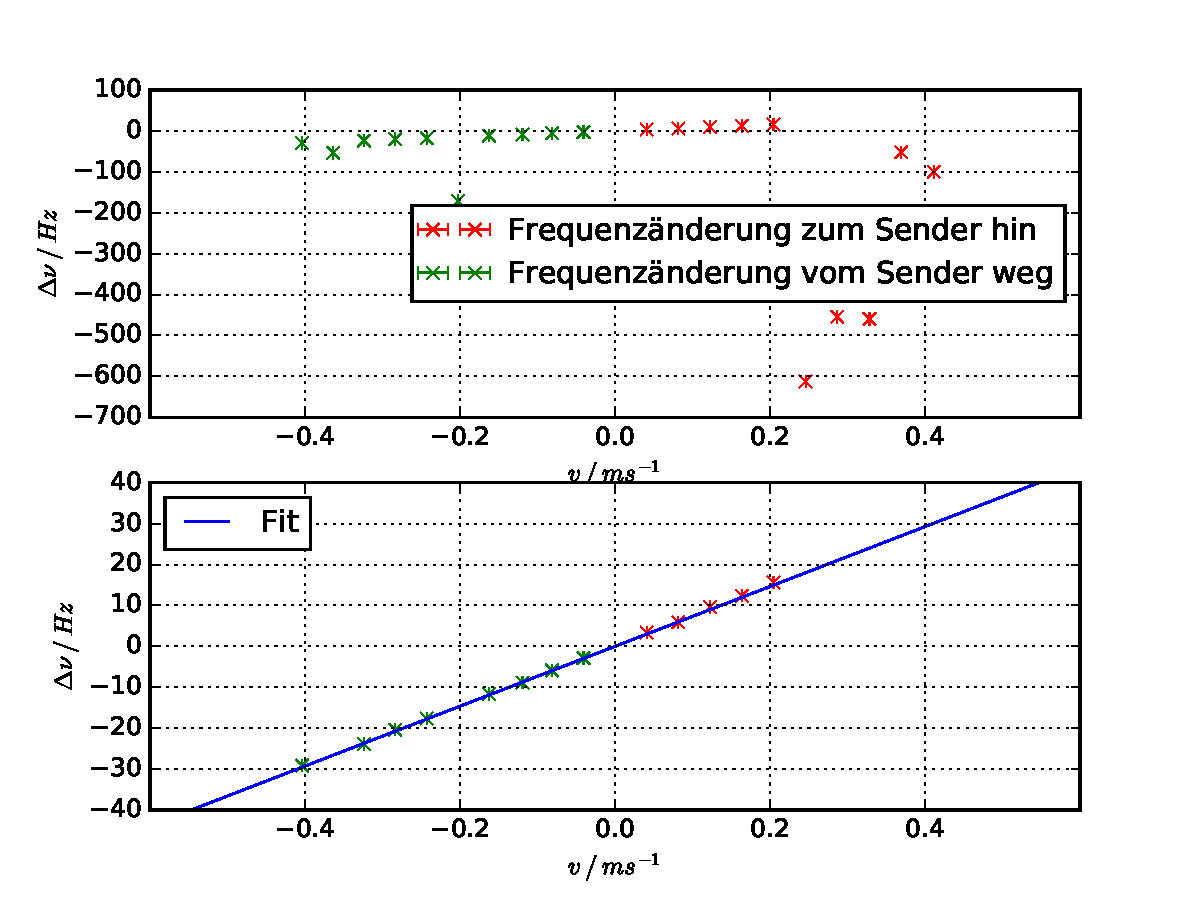
\includegraphics[width=0.8\textwidth]{plots/dplot.pdf}
  \caption{Frequenzänderung für einen bewegten Empfänger}
  \label{fig:d}
\end{figure}
%354.3946558999303+/-2.443400369412976
Aus dem Fit ergibt sich mit dem Zusammenhang \eqref{eqn:a} die
Schallgeschwindigkeit $c \approx (354,39 \pm 2,44)\; \frac{\symup{m}}{\symup{s}}$.

\FloatBarrier
\subsection{Frequenzänderung des bewegten Reflektors}
% 347.9546534809624+/-1.0812460480766823] vor wärts
% -353.20864806363323+/-11.01047986738201 rueckwärts

Auch hier wurde mit Formel \eqref{eqn:fit} ein Fit durchgeführt. Daraus ergibt
sich für den Reflektor der sich von der Quelle weg bewegt mit Gleichung \eqref{eqn:a}
die Schallgeschwindigkeit $c \approx ( 353,2 \pm 11)\; \frac{\symup{m}}{\symup{s}}$
und für den Reflektor der sich auf die Quelle zu bewegt ergibt sich
$c \approx (347,95 \pm 1,08)\; \frac{\symup{m}}{\symup{s}}$.
\begin{figure}
  \centering
  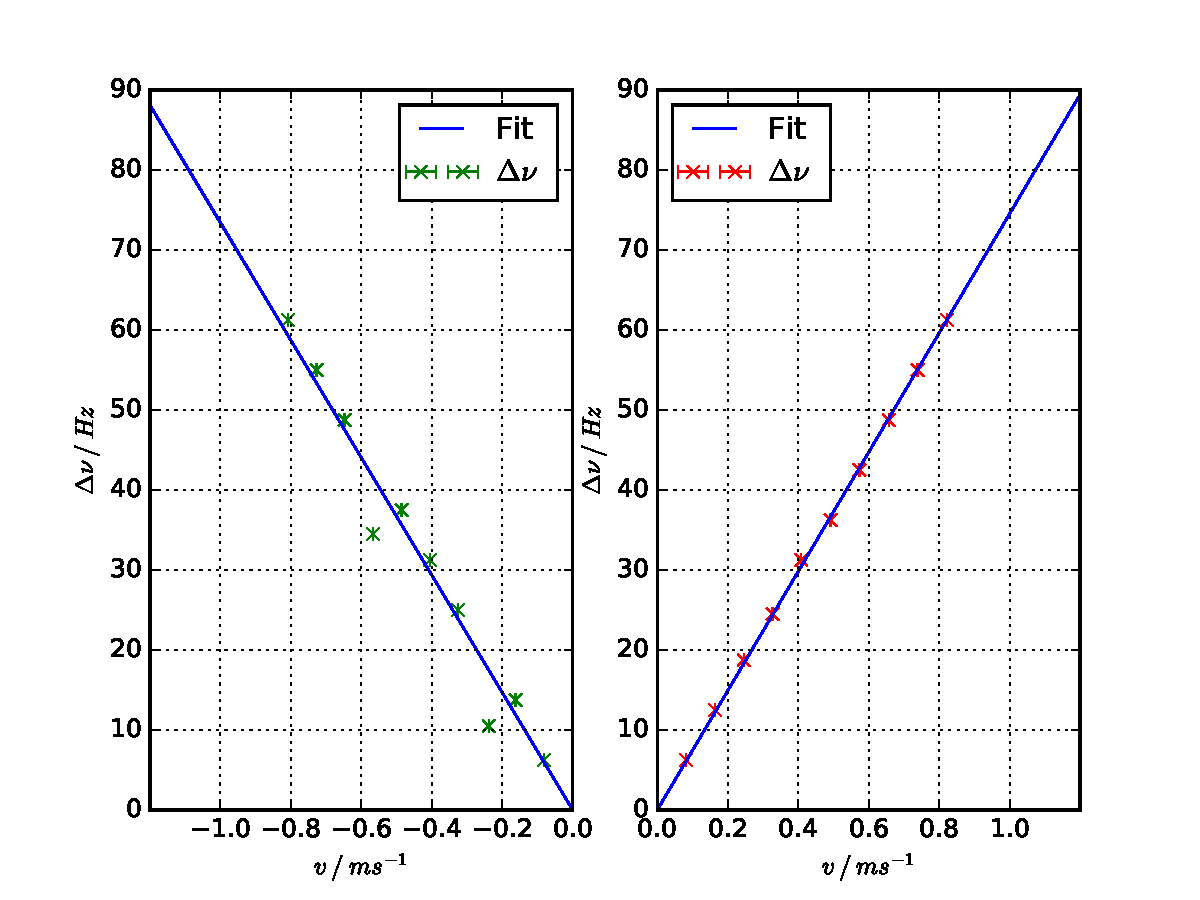
\includegraphics[width = 0.8\textwidth]{plots/eplot.pdf}
  \caption{Frequenzänderung bei einem bewegten Reflektor}
  \label{fig:e}
\end{figure}



























%
